\section{Groups} 

\subsection{Group-Like Structures} 

  Now the endowment of some structures gives rise to the following. Usually, we will start with the most general algebraic structures and then as we endow them with more structure, we can prove more properties. 

  \begin{definition}[Semigroup]
    A \textbf{semigroup} $(S, *)$ is a set $S$ with an associative binary operation. 
  \end{definition} 

  \begin{definition}[Monoid]
    A \textbf{monoid} $(M, *)$ is a semigroup with an identity element $1 \in M$ such that given a $m \in M$
    \begin{equation}
      1 * m = m * 1 = m
    \end{equation}
  \end{definition}

  Groupoids aren't necessarily that interesting, but there are cases in which semigroups and monoids come up. 

  \begin{example}[Continuous Time Markov Chain]
    Let $(\Omega, \mathcal{F}, \mathbb{P})$ be a probability space and $(S, \mathcal{S})$ a measurable space. Then, a homogeneous continuous-time Markov chain is a stochastic process $\{X_t\}_{t \geq 0}$ taking values in $S$ (i.e. $X_t: \Omega \rightarrow S$) satisfying the \textbf{Markov property}: for every bounded measurable $f$ and and $t, s \geq 0$, 
    \begin{equation}
      \mathbb{E}[ f(X_{t + s}) \mid \{X_r\}_{r \leq t} ] = \mathbb{E}[ f(X_{t + s}) \mid X_t ] = (P_s f)(X_t)
    \end{equation}
    The set $\{P_t\}_{t \geq 0}$ is called the \textbf{Markov semigroup}. 
  \end{example} 

  \begin{example}[Monoid of Transformations]
    Given a set $S$, consider the set of all functions $f: S \rightarrow S$. This forms a monoid with the identity function $f(x) = x$ as the identity element. Proof of associativity is shown in my set theory notes. 
  \end{example} 

  \begin{theorem}[Cardinality of Monoid of Transformations]
    If $|S| = n$, then the monoid of transformations has cardinality $n^n$. 
  \end{theorem}

  \begin{example}
    Let $S$ be any nonempty set. Then $(2^S, \cup, \emptyset)$ and $(2^S, \cap, S)$ are monoids. 
  \end{example}

  We first should ask whether the identity is unique in a monoid. It turns out it is. 

  \begin{lemma}[Uniqueness of Monoid Identity]
    The identity $1$ of a monoid $M$ is unique. 
  \end{lemma}
  \begin{proof}
    Assume not, i.e. there are 2 identities $1 \neq 1^\prime$. But then 
    \begin{equation}
      1 = 1 1^\prime = 1^\prime \implies 1 = 1^\prime
    \end{equation}
    where the implication follows from transitivity of equivalence relations. 
  \end{proof} 

  \begin{definition}[Submonoid]
    Given a monoid $(M, \ast)$, let $M^\prime \subset M$. If the restriction of $\ast$ to $M^\prime \times M^\prime$ is closed in $M^\prime$, then we can define the \textbf{submonoid} $(M^\prime, \ast)$. 
  \end{definition} 

  \begin{theorem}[Identities of Submonoids]
    If $M^\prime$ with identity $1^\prime$ is a submonoid of $M$ with identity $1$, Then $1 = 1^\prime$. 
  \end{theorem}
  \begin{proof}
    Assume not. $1^\prime \in M$, which means that 
  \end{proof}

\subsection{Groups}

  \begin{definition}[Group]
    A \textbf{group} is a monoid where every element has an inverse element. That is, $(G, *)$ is a set with binary operation having the properties of closure, associativity, existence of an identity and existence of inverses, in the following order: 
    \begin{enumerate}
      \item $x, y \in S \implies x*y, \;y*x \in G$ but not necessarily $x*y  = y*x$
      \item $a*(b*c) = (a*b)*c \; \forall a, b, c \in G$
      \item $\exists I \in G : x*I = I*x = x \; \forall x \in G $
      \item $\forall x \in G \; \exists x^{-1} \in G : x * x^{-1} = x^{-1} * x = I$
    \end{enumerate}
  \end{definition}

  \begin{proposition}[Uniqueness of Identity and Inverse]
    The identity and the inverse is unique, and for any $a, b$, the equation $x*a = b$ has the unique solution $x = b* a^{-1}$.
  \end{proposition}
  \begin{proof}
     Assume that there are two identities of group $(G,*)$, denoted $I_{1}, I_{2}$, where $I_{1} \neq I_{2}$. According to the properties of identities, $I_{1} = I_{1} * I_{2} = I_{2} \implies I_{1} = I_{2}$. \\
    As for uniqueness of a inverses, let $a$ be an element of $G$, with its inverses $a_{1}^{-1}, a_{2}^{-1}$. Then, 
    \begin{align*}
      a * a_{1}^{-1} = I & \implies a_{2}^{-1} * \Big(a * a_{1}^{-1} \Big)= a_{2}^{-1} * I \\
       & \implies \Big(a_{2}^{-1} * a \Big) * a_{1}^{-1} = a_{2}^{-1} \\
       & \implies I * a_{1}^{-1} = a_{2}^{-1}
    \end{align*}
    Since the inverse is unique, we can operate on each side of the equation $x*a = b$ to get $x*a*a^{-1} = b*a^{1} \implies x * I = x = b*a^{-1}$. Clearly, the derivation of this solution is unique since the elements that we have operated on are unique.
  \end{proof} 

  \begin{definition}[Subgroup]
    Given group $(G, \ast)$ and $(G^\prime, \ast)$ with the same operations, $G^\prime$ is a \textbf{subgroup} of $G$ if $G^\prime \subset G$. 
  \end{definition}

  \begin{definition}[Group Homomorphism]
    Let $(M, \circ)$ and $(N, *)$ be two sets with their respective operations. The mapping $f: (M, \circ) \longrightarrow (N, *)$ is a \textbf{group homomorphism} if
    \begin{equation}
      f(a \circ b) = f(a) * f(b) \; \forall a, b \in M
    \end{equation}
    A homomorphism is a \textbf{group isomorphism} if and only if it is bijective, which is also stated by saying that $M$ and $N$ are \textbf{isomorphic (as groups)}, denoted $M \simeq N$. A homomorphism from structure $G$ to itself is called an \textbf{endomorphism}, and an endomorphism that is also an isomorphism is called an \textbf{automorphism}. 
  \end{definition}

  \begin{example}[Exponential Map]
    The map $a \mapsto 2^{a}$ is an isomorphism between $(\mathbb{R}, +)$ and $(\mathbb{R}^{+}, \times)$ since 
    \begin{equation}
      2^{a+b} = 2^a \times 2^b
    \end{equation} 
    which is proved in my real analysis notes when constructing the exponential map on the reals. 
  \end{example} 

  Notice that given any set $S$, we can define the set of all functions $f: S \rightarrow S$ as a monoid. What if we consider the set of all invertible functions? This by definition means bijective functions, and so consider this subset.  

  \begin{definition}[Transformation Group]
    Given a set $S$, the \textbf{transformation group}, or \textbf{symmetric group}, of $S$ is the group of all bijective maps from $S$ to itself. 
  \end{definition}

  Therefore, we can see that \textit{every} set, whether a group or not, has an associated group of transformations acting on that set. 

  \begin{theorem}[Quotient Maps are Homomorphisms]
    Given a group $(G, \ast)$ with an equivalence relation $\sim$, the quotient map $\iota: (G, \ast) \rightarrow (G/\sim, \ast^\prime)$, which is defined as the mapping satisfying 
    \begin{equation}
      \iota(a) *^\prime \iota(b) \equiv \{ a \ast b \} 
    \end{equation}
    for all $a, b \in G$, is a group homomorphism. 

    \begin{figure}[H]
      \centering 
      \begin{tikzcd}
        G \times G \arrow[r, "\ast"] \arrow[d, "\iota"] & G \arrow[d, "\iota"] \\ 
        (G/\sim) \times (G/\sim) \arrow[r, "\ast^\prime"] & G/\sim
      \end{tikzcd}
      \caption{The commutative diagram is equivalent to the claim that $\iota$ is a homomomorphism.} 
      \label{fig:quotient_homomorphism}
    \end{figure}
  \end{theorem}
  \begin{proof}
    
  \end{proof}

  \begin{definition}[Abelian Group]
    An \textbf{abelian group} $(A, +)$ is a group where $+$ is commutative.\footnote{Note that I switched the notation from $\ast$ to $+$. By convention and to avoid confusion, $+$ denotes commutative operations. }
  \end{definition}

  \begin{example}[Abelian Groups]
    Here are some examples. 
    \begin{enumerate}
      \item $\mathbb{Z}, \mathbb{Q}, \mathbb{R}$ are all abelian groups with respect to addition. $\mathbb{Q}^{*} \equiv \mathbb{Q} \setminus \{0\}$ and $\mathbb{R}^{*} \equiv \mathbb{R} \setminus \{0\}$ are abelian groups with respect to multiplication.
      \item The set of all functions on a given interval $F[a,b]$ is abelian with respect to addition, defined as $(f+g)(x) \equiv f(x) + g(x)$. 
    \end{enumerate}
  \end{example}

\subsection{Generating Sets}

  A group $G$ may be very abstract and complicated, and so working with all its elements can be a bit painful. It would be more useful to work with a smaller subset $S$ of $G$ that can completely characterize $G$.\footnote{Note that this is similar to the basis that generates a topology.} We would like to formalize this notion, which will be very useful later on. 

  \begin{definition}[Word]
    A \textbf{word} is any written product of group elements and inverses. They are generally in the form
    \begin{equation}
      s_{1}^{\epsilon_{1}} s_{2}^{\epsilon_{2}} s_{3}^{\epsilon_{3}}... s_{k}^{\epsilon_{k}}, \text{ where} e_i \in \mathbb{Z}
    \end{equation} 
    e.g. given a set $\{x,y,z\}$, $x y, x z^{-1} y y x^{-2},...$ are words. 
  \end{definition}

  \begin{definition}[Generating Set]
    The \textbf{generating set} $\langle S \rangle$ of a group $G$ is a subset of $G$ such that every element of the group can be expressed as a word of finitely many elements under the group operations. The elements of the generating set are called \textbf{generators}.
  \end{definition}

  \begin{definition}[Cyclic Group]
    A \textbf{cyclic group}, denoted $C_{n}$, is a group generated by a single element. In a \textbf{finite cyclic group}, there exists a $k \in \mathbb{N}$ such that $g^{k} = g^{0} = 1$ (or in additive notation, $kg = 0g = 0$), where $g$ is the generator. A \textbf{finitely generated group} is a group generated by a finite number of elements. In \textbf{infinite cyclic groups}, all elements are distinct for distinct $k$. 
  \end{definition}

  \begin{example}[Roots of Unity]
    The $n$th roots of unity in $\mathbb{C}$ is a cyclic group of order $n$. 
  \end{example}

  \begin{example}[Discrete Rotations]
    Another representation of a cyclic group of $n$th order is the set of discrete angular rotations in $SO(2)$, in the form of 
    \begin{equation}
      R =  \bigg\{ \begin{pmatrix}
      \sin{\theta} & \cos{\theta} \\
      \cos{\theta} & -\sin{\theta}
      \end{pmatrix}\; \bigg| \; \theta \in \Big\{\frac{2 \pi}{n} k\Big\}_{k = 0}^{n-1} \bigg\}
    \end{equation}
  \end{example}

  \begin{example}
    $\mathbb{Z}$ is an infinite cyclic group with generator $1$. Furthermore, $\mathbb{Z}/m\mathbb{Z}$ is a finite cyclic group with generator $1$. In fact, the generator of $\mathbb{Z}/m\mathbb{Z}$ can be any integer relatively prime to $m$ (and less than $m$). 
  \end{example}

  \begin{theorem}[Transpositions]
    The set of all \textbf{transpositions} forms a generating set of $S_{n}$. 
  \end{theorem}

  It is actually a fact that every finite cyclic group of order $m$ is isomorphic to $\mathbb{Z}/m\mathbb{Z}$. Every infinite cyclic group is isomorphic to $\mathbb{Z}$. This implies that any two cyclic group of the same order are isomorphic, since we can define a mapping $f:a\longrightarrow b$, where $a$ and $b$ are generating elements of their respective groups. 

  \begin{example}
    Dih$(3) \simeq S_{3}$, since permutations of the vertices of a triangle are isomorphic to a permutations of a 3-element set. 
  \end{example}

  \begin{definition}
    The \textbf{free group} $F_{S}$ over a given set $S$ consists of all words that can be built from elements of $S$. Clearly, $S$ is the generating set of $F_{S}$. 
  \end{definition}

  Now for notational convenience, one method of specifying a group is to put it in the form
  \begin{equation}
    \big\langle \; S \; | \; R \;\big\rangle
  \end{equation}
  where $S$ is the generating set and $R$ is a set of relations. This is called the \textit{group presentation}. 

  \begin{example}[Group Presentations]
    The cyclic group of order $n$ could be presented as
    \begin{equation}
      \big\langle \; a \; | \; a^{n} = 1 \;\big\rangle
    \end{equation}
    Dih $(8)$, with $r$ representing a rotation by $45$ degrees in the direction of the orientation and $f$ representing a flip over any axis, is presented by
    \begin{equation}
      \big\langle \; \{ r, f\} \; | \; r^{8} = 1, f^{2} = 1, (r f)^{2} = 1 \;\big\rangle
    \end{equation}
  \end{example}

\subsection{Finite Symmetric Groups}

  \begin{definition}[Permutation Group]
    The \textbf{permutation group} is the set of all bijective transformations from any set $X$ to the same set, denoted either Sym$(X)$ or $S_n$. If $X = \{1, 2, 3 ,... , n\}$, known as the set of all permutations of $X$, with cardinality $n!$. 
  \end{definition}

  \begin{proposition}
    Every element in finite $S_{n}$ can be decomposed into a partition of cyclic rotations.
  \end{proposition}

  \begin{example}
    Listed.
    \begin{enumerate}
      \item $(1 2)$ is a mapping $1 \rightarrow 2,\; 2 \rightarrow 1$. 
      \item $(1 2 3)$ is a mapping $1\rightarrow 2,\; 2 \rightarrow 3,\; 3 \rightarrow 1$. 
      \item $(1 2 3) (4 5)$ is a mapping $1\rightarrow 2,\; 2 \rightarrow 3,\; 3 \rightarrow 1, \;4 \rightarrow 5, \;5 \rightarrow 4$. 
    \end{enumerate}
  \end{example}

  \begin{definition}
    The \textbf{conjugacy class} of $S_{n}$ correspond to the cycle structures of $S_{n}$. Two elements of $S_{n}$ are conjugate in $S_{n}$ if and only if they consist of the same number of disjoint cycles of the same lengths. 
  \end{definition}

  \begin{example}
    \begin{enumerate}
      \item $(1 2 3) (4 5)$ is conjugate to $(1 4 3) (2 5)$.
      \item $(1 2) (4 5)$ is not conjugate to $(1 4 3) (2 5)$. 
    \end{enumerate}
  \end{example}

  \begin{definition}
    The \textbf{signature} of a permutation is a homomorphism
    \begin{equation}
      \text{sgn}: S_{n} \longrightarrow \{1, -1\}
    \end{equation}
  \end{definition}

  \begin{proposition}
    The signature of a permutation changes for every transposition that is applied to it. 
  \end{proposition}

  \begin{definition}[Alternating Group]
    The \textbf{alternating group} of order $n$ is the set of all \textbf{even permutations} (permutations that have signature $1$) of $\{1, 2, ..., n\}$. It is denoted $A_{n}$ or Alt$(n)$ and its cardinality is $\frac{1}{2} n!$. Note that the set of odd permutations do not form a group, since the composition of two odd permutations (each having signature $-1$ is an even permutation. 
  \end{definition}

  \begin{example}[Low Order Symmetric Groups]
    \begin{enumerate}
      \item $S_{0}$ is the set of all permutations on the \textbf{null set}. $S_{1}$ is the set of all permutations on the \textbf{singleton set}. Both sets have cardinality 1 and the element is \textbf{trivial}. Note that $S_{1} = A_{1}$. 
      \item $S_{2}$ is a cyclic, abelian group of order 2 consisting of the identity permutation and the transposition of two elements. 
      \item $S_{3}$ is the first cyclic, nonabelian group, with order 6.$S \simeq \text{Dih}(3)$, which can be seen as the group of rotations and reflections on the equilateral triangle, and the elements of $S_{3}$ equate to permuting the vertices on the triangle. 
    \end{enumerate}
  \end{example}

  Now we move onto more geometric groups. 

  \begin{definition}
    A \textbf{polytope} in $n$-dimensions is a geometrical object with "flat sides, " called an n-polytope. It is a generalization of a polygon or a polyhedron to an arbitrary number of dimensions. 
  \end{definition}

  \begin{definition}
    A \textbf{n-simplex} is a n-polytope which is the n-dimensional convex hull of its $n+1$ vertices. Moreover, the $n+1$ vertices must be \textbf{affinely independent}, meaning that
    \begin{equation}
      \{u_1 - u_0, u_2 - u_0, ..., u_n - u_0 | \{u_i\}_{i=0}^{n} \text{ vertices} \}
    \end{equation}
    are linearly independent vectors that span the n-dimensional space. 
  \end{definition}

  \begin{definition}
    The \textbf{symmmetry group} of a geometrical object is the group of all transformations in which the object is invariant. Preserving all the relevant structure of the object. A common example of such groups is the \textbf{dihedral group}, denoted D$_{n}$ or Dih$(n)$, which is the group of symmetries of a n-simplex, which includes rotations and reflections. 
  \end{definition}

  \begin{example}
    We introduce some low order Dihedral groups. 
    \begin{enumerate}
      \item Dih$(3)$ is the group of all rotations and reflections that preserve the structure of the equilateral triangle in $\mathbb{R}^2$, a regular 2-simplex. 
      \begin{center}
      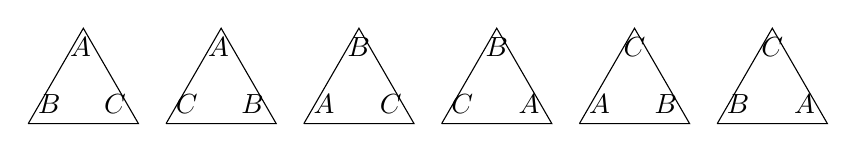
\begin{tikzpicture}[scale=0.7]
          \draw (-1,0)--(1,0)--(0,1.732)--(-1,0);
          \draw (-3.5,0)--(-1.5,0)--(-2.5,1.732)--(-3.5,0);
          \draw (-6,0)--(-4,0)--(-5,1.732)--(-6,0);
          \draw (4,0)--(6,0)--(5,1.732)--(4,0);
          \draw (1.5,0)--(3.5,0)--(2.5,1.732)--(1.5,0);
          \draw (6.5,0)--(8.5,0)--(7.5,1.732)--(6.5,0);
          \node[below] at (-5.05, 1.732) {$A$};
          \node[below] at (-2.55, 1.732) {$A$};
          \node[below] at (-0, 1.732) {$B$};
          \node[below] at (2.5, 1.732) {$B$};
          \node[below] at (5, 1.732) {$C$};
          \node[below] at (7.5, 1.732) {$C$};
          \node[above right] at (-6,0) {$B$};
          \node[above right] at (-3.5,0) {$C$};
          \node[above right] at (-1,0) {$A$};
          \node[above right] at (1.5,0) {$C$};
          \node[above right] at (4,0) {$A$};
          \node[above right] at (6.5,0) {$B$};
          \node[above left] at (-4.05,0) {$C$};
          \node[above left] at (-1.55,0) {$B$};
          \node[above left] at (0.95,0) {$C$};
          \node[above left] at (3.45,0) {$A$};
          \node[above left] at (5.95,0) {$B$};
          \node[above left] at (8.45,0) {$A$};
      \end{tikzpicture}
      \end{center}
      \item Dih$(4)$ is the group of all rotations and reflections that preserve the structure of the regular tetrahedron in $\mathbb{R}^{3}$. An incorrect, yet somewhat useful, way of visualizing this group is to imagine a square in $\mathbb{R}^{2}$. However, the points are not pairwise equidistant and therefore does not preserve symmetry between all points.
      \item Dih$(n)$ is similarly the group of all rotations and reflections that preserve the structure of a regular $(n-1)$-simplex in $\mathbb{R}^{n}$. 
    \end{enumerate}
  \end{example}

\subsection{Direct Product of Groups}

  \begin{definition}
    The \textbf{direct product} of two groups $G$ and $H$ is denoted
    \begin{equation}
      G \times H \equiv \{ (g, h)\;|\; g \in G, h \in H \}
    \end{equation}
    Note that the product need not be binary (nor must it be of finite arity). 
  \end{definition}

  \begin{definition}
    The \textbf{general affine group} is defined 
    \begin{equation}
      \text{GA}(V) \equiv \text{Tran}\,V \times \text{GL}(V)
    \end{equation}
  \end{definition}

  \begin{definition}
    The \textbf{Galileo Group} is the transformation group of spacetime symmetries that are used to transform between two reference frames which differ only by constant relative motion within the constructs of Newtonian physics. It is denoted 
    \begin{equation}
      \text{Tran}\;\mathbb{R}^{4} \times H \times \text{O} (3)
    \end{equation}
    where $H$ is the group of transformations of the form 
    \begin{equation}
      (x, y, z, t) \longmapsto (x+at, y+bt, z+ct, t)
    \end{equation}
  \end{definition}

  \begin{definition}
    The \textbf{Poincaré Group} is the symmetry group of spacetime within the principles of relativistic mechanics, denoted
    \begin{equation}
      G = \text{Tran}\; \mathbb{R}^{4} \times \text{O}_{3,1}
    \end{equation}
    where O$_{3,1}$ is the group of linear transformations preserving the polynomial 
    \begin{equation}
      x^{2} + y^{2} + z^{2} - t^{2}
    \end{equation}
  \end{definition}

\subsection{Classes of Groups}

  \subsubsection{General Linear and Affine Groups}

    \begin{definition}
      The \textbf{general linear group}, denoted GL$(V)$, is the set of all bijective linear mappings from $V$ to itself. Similarly, GL$_{n}(\mathbb{F})$, or GL $(n, \mathbb{F})$ is the set of all nonsingular $n \times n$ matrices over the field $\mathbb{F}$. Due to the same dimensionality of the following spaces, it is clear that GL$(V) \simeq$ GL$(\mathbb{F}^{n}) \simeq$ GL$_{n}(\mathbb{F})$. The \textbf{special linear group}, denoted SL$_{n} (\mathbb{F})$ or SL$(n, \mathbb{F})$, is the set of $n\times n$ matrices a with determinant $1$. SL$_{n}(\mathbb{F})$ is a subgroup of GL$_{n}(\mathbb{F})$, which is a subset of the ring of all $n \times n$ matrices over field $\mathbb{F}$, denoted $\mathbb{L}_{n}(\mathbb{F})$. 
    \end{definition}

    \begin{definition}
      The \textbf{general affine group} is the pair of all transformations
      \begin{equation}
        \text{GA} (V) \equiv \text{Tran}(V) \times \text{GL}(V)
      \end{equation}
    \end{definition}

  \subsubsection{Isometries}

    \begin{definition}
      The group of all translations in the space $V$ is denoted Tran$\,V$. Its elements are usually denoted as $t_{u}$, where $u$ is the vector that is being translated by. It can also be interpreted as shifting the origin by $-u$. It is clear that Tran$\,V \simeq V$. 
    \end{definition}

    \begin{definition}
      The \textbf{Euclidean group} of \textbf{isometries} in the Euclidean space $\mathbb{E}^{n}$ (with the Euclidean norm), denoted Isom$\, \mathbb{E}^{n}$ or $\mathbb{E}(n)$, consists of all distance-preserving bijections from $\mathbb{E}^{n}$ to itself, called \textbf{motions} or \textbf{rigid transformations}. It consists of all combinations of rotations, reflections, and translations. The \textbf{special Euclidean group} of all isometries that preserve the \textbf{handedness} of figures is denoted $\mathbb{SE}(n)$, which is comprised of all combinations rotations and translations called \textbf{rigid motions} or \textbf{proper rigid transformations}.
    \end{definition}

    \begin{definition}
      The \textbf{orthogonal group}, denoted O$(n)$ or O$_{n}$, consists of all isometries that preserve the origin, i.e. consists of rotations and reflections. The \textbf{special orthogonal group}, denoted SO$(n)$, is a subgroup of O$(n)$ consisting of only rotations. We can see that 
      \begin{equation}
        \text{O}(n)=\frac{\text{Isom}\, \mathbb{E}^{n}}{\text{Tran}\,V}
      \end{equation}
    \end{definition}

\subsection{Cayley's Theorem}

  \begin{lemma}
    Let $G$ be a group with $a \in G$. We define the map
    \begin{equation}
      \phi: G \longrightarrow G, \; \phi (x) = a x a^{-1}
    \end{equation}
    Then, $\phi$ is an automorphism of $G$. 
  \end{lemma}
  \begin{proof}
    The map $\psi: G \longrightarrow G, \; \psi(x) = a^{-1} x a$ is clearly the inverse of $\phi$, with $\phi \psi = \psi \phi = I$ for all $x \in G \implies \phi$ is bijective. Secondly, $\phi(x) \phi(y) = a x a^{-1} a y a^{-1} = a (x y) a ^{-1} = \phi (x y) \implies \phi$ preserves the group structure. 
  \end{proof}

  \begin{theorem}[Cayley's Theorem]
    Every group $G$ is isomorphic to a subgroup of its symmetric group. If $G$ is finite, then so is Sym$(G)$, so every finite group is a subgroup of $S_{n}$, for some $n$.
  \end{theorem}
  \begin{proof}
    Let $H =$ Sym$(G)$. We define the map
    \begin{equation}
      \phi: G \longrightarrow H
    \end{equation}
    by the following rule. For $a \in G$, map it to permutation $\sigma = \phi (a) \in H$ defined as $\sigma(g) = a g$ for all $g \in G$. Note that given an $a \in G$, $a g$ must also be in $G$, meaning that a corresponding $\sigma \in H$ exists. It is sufficient to prove that $\phi$ is an isomorphism onto its image. We first prove injectivity. Given $a \neq b \in G$, $\phi(a)=\sigma, \phi(b) = \tau$. Assume $\sigma = \tau \implies a = a e =  \sigma(e) = \tau (e) = b e = b \implies a = b$, a contradiction. We now check that $\phi(a b) = \phi(a) \phi(b)$. Given $g \in G, \phi(a) \phi(b) (g) = \phi(a) (bg) = a(bg)= (ab) g = \phi(ab) (g).$
  \end{proof}

\subsection{Group Actions}

  \begin{definition}
    Let $G$ be a group, $X$ a set. Then, a (left) group action of $G$ on $X$ is a function: 
    \begin{equation}
      \varphi: G \times X \longrightarrow X, \; (g,x) \longmapsto \varphi(g,x)
    \end{equation}
    satisfying two axioms:
    \begin{enumerate}
      \item Identity. $\forall x \in X, \varphi(e, x) = x$. 
      \item Compatibility. $\forall g, h \in G \text{ and } \forall x \in X, \varphi(gh, x) = \varphi(g, \varphi(h, x))$.
    \end{enumerate}
    The group $G$ is said to \textbf{act on} $X$. $X$ is called a \textbf{G-set}. The two axioms, furthermore, imply that for every $g \in G$, the function that maps $x \in X$ to $ \varphi(g, x) \in X$ is a bijective map, since the inverse is the function mapping $x \mapsto \varphi(g^{-1}, x)$. \\
    $(g, x)$ can be interpreted as the element $g$ in the transformation group $G$ acting on an element $x$ in $X$.
  \end{definition}

  \begin{example}
    Isom$\,\mathbb{R}^{3}$ acts on $\mathbb{R}^{3}$ since every element $g \in$ Isom$\,\mathbb{R}^{3}$ acts on the entire space $\mathbb{R}^{3}$. 
  \end{example}

  \begin{example}
    $S_n$ acts on $\{1, 2, ..., n\}$by permuting its elements.
  \end{example}

  \begin{example}
    The GA$(V)$ acts transitively on the points of an affine space.
  \end{example}

  \textbf{Equivalent Interpretation of Group Actions}
  Note that this group action $G$ on space $X$ identifies a group homomorphism into the group of automorphisms of that space. Given an abstract group element $g \in G$, $\varphi(g, \cdot): X \longrightarrow X$ is defined accordingly, where $\varphi(g, \cdot) \in $ Aut$(X)$. So alternatively, we can interpret a group action as a homomorphism from $G$ to Aut$(X)$. 
  \begin{equation}
    \phi: G \longrightarrow \text{Aut}(X), \; g \mapsto \phi(g) = \varphi(g,\cdot)
  \end{equation}

  \begin{definition}
    A group action on a finite-dimensional vector space $X$ is called a \textbf{representation} of that group. 
  \end{definition}

\subsection{Equivalence and Congruence}

  \begin{definition}
    A transformation group $G$ is called \textbf{transitive} if for any $x, y \in X$, there exists a $\phi \in G$ such that $y = \phi(x)$. 
  \end{definition}

  \begin{example}
    Tran$(V)$ and GA$(V)$ are transitive groups. 
  \end{example}

  \begin{definition}
    Let $X$ be a set and $G$ its transformation group on $X$. The way we define $G$ determines the \textbf{geometry} of $X$. More specifically, a figure $F_{1} \subset X$ is \textbf{equivalent} or \textbf{congruent} to $F_{2} \subset X$ iff there exists $\phi \in G$ such that $F_{2} = \phi (F_{1})$ (or equivalently, $F_{1} = \phi (F_{2})$). This is an equivalence relation since
    \begin{enumerate}
      \item $F \sim F$. 
      \item $F \sim H \implies H \sim F$. 
      \item $F \sim H, H \sim K \implies F \sim K$
    \end{enumerate}
    Two figures that are in the same equivalence class are known to be \textbf{congruent} with respect to the geometry of $X$ induced by $G$. 
  \end{definition}

  Clearly, if two figures are congruent in Euclidean geometry, then they are congruent in Affine geometry, since E$(n) \subset$ GA$(n)$. 

\subsection{Cosets and Lagrange's Theorem}

  \begin{definition}
    Given a group $G$ and a subgroup $H$, $g_1$ and $g_2$ are congruent modulo $H$, denoted $g_1 \equiv g_2 \pmod{H}$. The equivalence classes are known as \textbf{cosets}. A coset of somprised of all the products obtained by multiplying each element of $H$ by a particular element in $G$. Since group multiplication is not necessarily commutative, we must distinguish between right and left cosets. 
    \begin{enumerate}
      \item A \textbf{left coset} is 
        \begin{equation}
          g H \equiv \{g h \;| \;h \in H \} 
        \end{equation}
      \item A \textbf{right coset} is 
        \begin{equation}
          H g \equiv \{h g \;|\; h \in H \}
        \end{equation}
    \end{enumerate}
    It is easy to see that the cosets form a partition of the set $X$, with each coset of the same cardinality. 
  \end{definition}

  \begin{definition}
    A subgroup $N \subset G$ is a \textbf{normal subgroup} iff the left cosets equal the right cosets. Every subgroup of an abelian group is normal. 
  \end{definition}

  \begin{theorem}[Lagrange's Theorem]
    Let $G$ be a finite group and $H$ its subgroup. Then 
    \begin{equation}
      |G| = |G:H| |H|
    \end{equation}
    where $|G:H|$ is the number of cosets in $G$. 
  \end{theorem}

  \begin{corollary}
    The order of a subgroup of a finite group divides the order of the group. 
  \end{corollary}

  \begin{definition}
    The order of an element is the order of the cyclic subgroup that it generates. 
  \end{definition}

  \begin{corollary}
    The order of any element of a finite group divides the order of the group. 
  \end{corollary}

  \begin{corollary}
    Every finite group of a prime order is cyclic. 
  \end{corollary}

  \begin{theorem}[Fermant's Little Theorem]
    Let $p$ be a prime number. The multiplicative group $\mathbb{Z}_{p} \setminus \{0\}$ of the field $\mathbb{Z}_{p}$ is an abelian group of order $p-1 \implies g^{p-1} = 1$ for all $g \in \mathbb{Z}_{p} \setminus \{0\}$. So,
    \begin{equation}
      a^{p-1} \equiv 1 \iff a^{p} \equiv a \pmod{p}
    \end{equation}
  \end{theorem}

  \begin{corollary}
    If $|G| = n$, then $g^{n} = e$ for all $g \in G$. 
  \end{corollary}

  \begin{definition}
    \textbf{Euler's Totient Function}, denoted $\varphi(n)$, consists of all the numbers less than or equal to $n$ that are coprime to $n$. 
  \end{definition}

  \begin{theorem}[Euler's Theorem (Generalization of Fermant's Little Theorem)]
    For any $n$, the order of the group $\mathbb{Z}_{n} \setminus \{0\}$ of invertible elements of the ring $\mathbb{Z}_{n}$ equals $\varphi(n)$, where $\varphi$ is Euler's totient function. In other words with $G = \mathbb{Z}_{n} \setminus \{0\}$, 
    \begin{equation}
      a^{\varphi(n)} \equiv 1 \pmod{n}, \; \text{ where $a$ is coprime to $n$}
    \end{equation}
  \end{theorem}

  \begin{example}
    In $\mathbb{Z}_{125} \setminus \{0\}$, $\varphi(125) = 125 - 25 = 100 \implies 2^{100} \equiv 1 \pmod{125}$
  \end{example}

  \begin{definition}
    Let $G$ be a transformation group on set $X$. Points $x, y \in X$ are equivalent with respect to $G$ if there exists an element $g \in G$ such that $y = g x$. This has already been defined through the equivalence of figures before. This relation splits $X$ into equivalence classes, called \textbf{orbits}. Note that cosets are the equivalence classes of the transformation group $G$; oribits are those of $X$. We denote it as
    \begin{equation}
      Gx \equiv \{ g x \;|\;g \in G \}
    \end{equation}
  \end{definition}

  By definition, transitive transformation groups have only one orbit.

  \begin{definition}
    The subgroup $G_{x} \subset G$, where $G_{x} \equiv \{ g \in G | g x = x\}$ is called the \textbf{stabilizer} of $x$.
  \end{definition}

  \begin{example}
    The orbits of $O(2)$ are concentric circles around the origin, as well as the origin itself. The stabilizer of the point $p \neq 0$ is the identity and the reflection across the line $??$. The stabilizer of $0$ is the entire $O(2)$.
  \end{example}

  \begin{example}
    The group $S_n$ is transitive on the set $\{1, 2, ..., n\}$. The stabilizer of $k, (1 \leq k \leq n)$ is the subgroup $H_{k} \simeq S_{n-1}$, where $H_k$ is the permutation group that does not move $k$ at all. 
  \end{example}

  \begin{theorem}
    There exists a 1-to-1 injective correspondence between an orbit $G_x$ and the set $G / G_{x}$ of cosets, which maps a point $y = g x \in G x $ to the coset $g G_x$. 
  \end{theorem}

  \begin{definition}
    The \textbf{length of an orbit} is the number of elements in it. 
  \end{definition}

  \begin{corollary}
    If $G$ is a finite group, then 
    \begin{equation}
      |G| = |G_x| |G x|
    \end{equation}
    In fact, there exists a precise relation between the stabilizers of points of the same orbit, regardless of $G$ being finite or infinite: 
    \begin{equation}
      G_{g x} = g G_{x} g^{-1}
    \end{equation}
  \end{corollary}

\subsection{Abelian Groups}

  First, note that the successive addition of elements of an additive abelian group can be represented by integer multiplication. 
  \begin{equation}
    x + x + ... + x = n x, \; n \in \mathbb{Z}
  \end{equation}
  Similarly, we can take the integer power of an element to represent successive multiplication in a multiplicative abelian group. 

  \begin{proposition}
    It is easy to check that in an additive abelian group $A$, with $a, b \in A$ and $k, l \in \mathbb{Z}$, 
    \begin{align}
      & k (a + b) = k a + k b \\
      & (k + l) a = k a + l a \\
      & (k l) a = k (l a)
    \end{align}
    which implies
    \begin{equation}
      k(a - b) = k a - k b, \; (k - l) a = k a - l a
    \end{equation}
  \end{proposition}

  \begin{definition}
    For any subset $S \subset A$, the collection of all linear combinations 
    \begin{equation}
      k_1 a_1 + k_2 a_2 + ... + k_n a_n, \; k_i \in \mathbb{Z}, a_i \in S
    \end{equation}
    is the smallest subgroup of $A$ containing $S$, called the \textbf{subgroup generated by $S$} and denoted $\langle S \rangle$. If $\langle S \rangle = A$, then we say that $A$ is \textbf{generated} by $S$, or that $S$ is a \textbf{generating set} of $A$. 
  \end{definition}

  \begin{definition}
    An abelian group that has a finite generating set is called \textbf{finitely generated}. Finitely generated abelian groups are similar to finite dimensional vector spaces. 
  \end{definition}

  \begin{definition}
    A system $\{ a_1, a_2, ..., a_n\}$ of elements of a group $A$ is called \textbf{linearly independent} if $k_1 a_1 + k_2 a_2 + ... + k_n a_n = 0 \implies k_1, k_2, ..., k_n = 0$. A system of linear independent elements that generates $A$ is called a \textbf{basis}. 
  \end{definition}

  Note that every finite dimensional vector has a basis, but not every finitely generated abelian group has one. For example, $(\mathbb{Z}_n, +)$ is generated by one element, but it has no basis since every element $a \in \mathbb{Z}_n$ satisfies the nontrivial relation $n a = 0$. 

  \begin{definition}
    A finitely generated abelian group is \textbf{free} if it has a basis. 
  \end{definition}

  \begin{theorem}
    All bases of a free abelian group $L$ contain the same number of elements. 
  \end{theorem}

  \begin{definition}
    The \textbf{rank} of a free abelian group $L$ is the number of elements in its basis. It is denoted rk$L$. The zero group is regarded as a free abelian group of rank $0$. 
  \end{definition}

  \begin{theorem}
    Every free abelian group $L$ of rank $n$ is isomorphic to the group $\mathbb{Z}^n$ of integer rows of length $n$. 
  \end{theorem}

  \begin{theorem}
    Every subgroup $n$ of a free abelian group $l$ of rank $n$ is a free abelian group of rank $ \leq n$. 
  \end{theorem}

  Note that unlike a vector space, a free abelian group of positive rank contains subgroups of the same rank that do not conside with the whole group. For example, the subgroup $m \mathbb{Z} \subset \mathbb{Z}, m > 0$ has rank $1$, just as the whole group. 

  Moreover, a free abelian group of rank $n$ can be embedded as a subgroup into an $n$-dimensional Euclidean vector space $E^n$. To do this, let $\{e_1, e_2, ..., e_n\}$ be a basis of $E^n$. Then, the subgroup generated by these basis vectors is the set of vectors with integer components, which is a free abelian group of rank $n$. This subgroup obtained as such is called a \textbf{lattice} in $E^n$. 

  \begin{definition}
    A subgroup $L \subset E^n$ is \textbf{discrete} if every bounded subset of $E^n$ contains a finite number of elements in $L$. Clearly, every lattice is discrete, and a subgroup generated by a linearly independent system of vectors (i.e. a lattice in a subspace of $E^n$) is discrete. 
  \end{definition}

  \begin{proposition}
    A subgroup $L \subset E^n$ is discrete if and only if its intersection with any neighborhood of $0$ consists of $0$ itself. 
  \end{proposition}

  \begin{theorem}
    Every discrete subgroup $L \subset E^n$ is generated by a linearly independent system of vectors of $E^n$. 
  \end{theorem}

  \begin{corollary}
    A discrete subgroup $L \subset E^n$ whose linear span coincides with $E^n$ is a lattice in $E^n$. 
  \end{corollary}

  Lattices in $E^3$ play an important role in crystallography since the defining feature of a crystal structure is the periodic repetition of the configuration of atoms in all three dimensions. More explicitly, let $\Gamma$ be the symmetry group of the crystal structure and let $\mathcal{L}$ be the group of all vectors $a$ such that the parallel translation $t_a \in \Gamma$. Then, $\mathcal{L}$ is a discrete subgroup of $E^n$ and thus, is a lattice in $E^3$. More specifically, we can present 
  \begin{equation}
    \Gamma \equiv \text{Dih}\,C \times \mathcal{L}
  \end{equation}
  where Dih$\, C$ is the Dihedral group of the crystal structure that preserves its lattices. 

  \begin{definition}
    An \textbf{integral elementary row transformation} of a matrix is a transformation of one of the following three types: 
    \begin{enumerate}
      \item adding a row multiplied by an integer to another row
      \item interchanging two rows
      \item multiplying a row by $-1$ 
    \end{enumerate}
    An \textbf{integral elementary column transformation} is defined similarly. 
  \end{definition}

  \begin{proposition}
    Every integral rectangular matrix $C = (c_{i j})$ can be reduced by integral elementary row transformations to the diagonal matrix diag$(u_1, ..., u_p)$, where $u_1, u_2, ..., u_p \geq 0$ and $u_i | u_{i+1}$ for $i = 1, 2, ..., p -1$. 
  \end{proposition}

  \begin{example}
    The following matrix can be reduced (with a few steps now shown) to the stated form. 
    \begin{equation}
    \begin{pmatrix} 2&6&2 \\ 2&3&4 \\ 4&2&4 \end{pmatrix} \rightarrow 
    \begin{pmatrix} 2&3&4 \\ 0&-3&2 \\ 4&2&4 \end{pmatrix} \rightarrow
    \begin{pmatrix} 1&0&0 \\ 0&6&14 \\ 0&8&12 \end{pmatrix} \rightarrow
    \begin{pmatrix} 1&0&0 \\ 0&2&0 \\ 0&0&20\end{pmatrix}
    \end{equation}
    where $1|2$ and $2|20$. 
  \end{example}

  Note that for $n \times 1$ or $1 \times n$ matrices, this procedure is precisely the Euclidean algorithm that produces the GCD of $n$ integers. 

  \begin{proposition}
    Given square integral matrix $C$ with  reduced form diag$(u_1, ..., u_p)$, 
    \begin{equation}
      u_i = \frac{d_i}{d_{i-1}}
    \end{equation}
    where $d_i$ is the GCD of the minors of order $i$ of the original matrix $C$. Recall that a minor of a matrix is the determinant of the matrix with one of its rows and columns removed. $d_0$ is assumed to equal $1$. This implies that the numbers $u_1, u_2, ..., u_p$, along with the reduced form, are uniquely determined by $C$. 
  \end{proposition}

  \begin{theorem}
    For any subgroup $N$ of a free abelian group $L$ of rank $n$, there exists a basis $\{e_1, ..., e_n\}$ of $L$ and natural numbers $u_1, ..., u_m, \; (m \leq n)$, such that $\{u_1 e_1, ..., u_m e_m\}$ is a basis fo the group $N$ and $u_i | u_{i+1}$ for $i = 1, 2, ..., m-1$. 
  \end{theorem}
    
